\section{Tomita's Alchemy}

\begin{figure}[htbp]
\centering
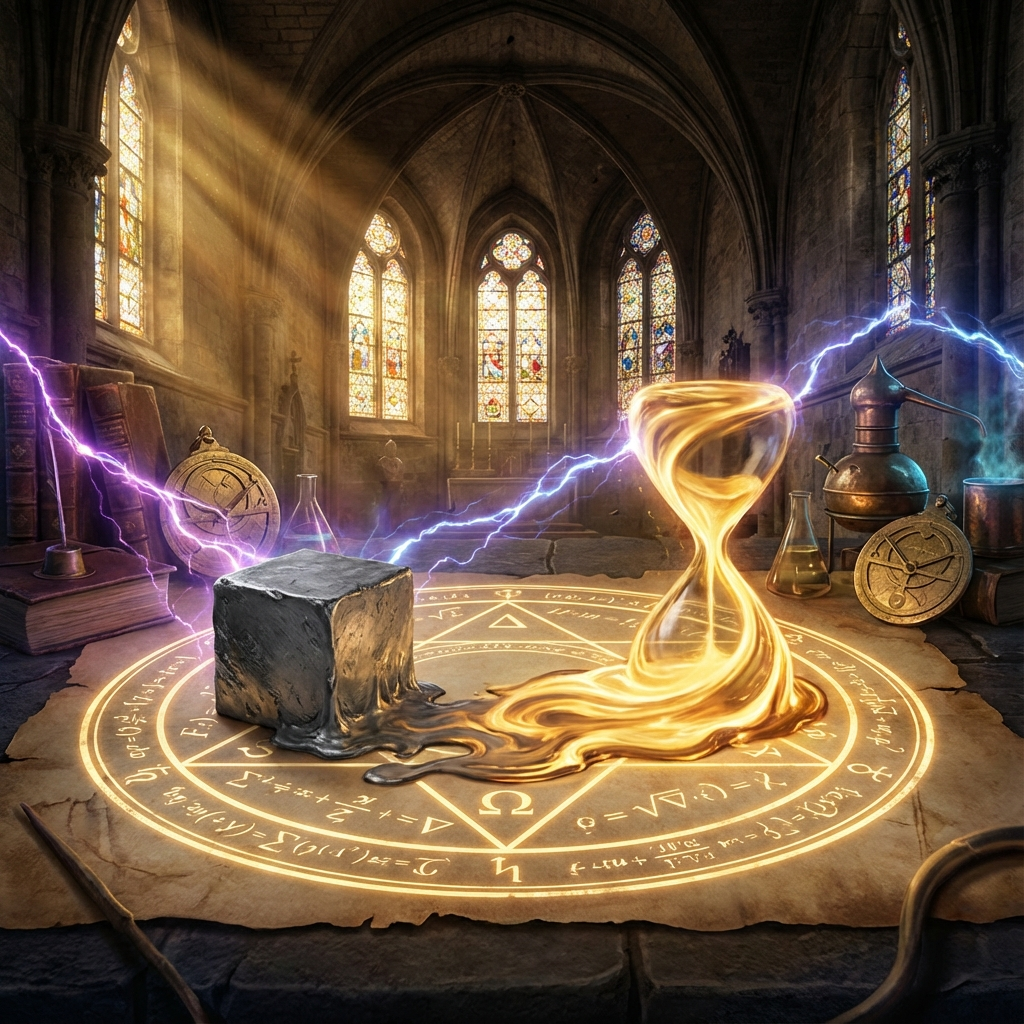
\includegraphics{assets/ch06_tomita_alchemy_1765302388187.png}
\caption{Tomita Alchemy}
\end{figure}

\begin{quote}
``Ancient alchemists tried to extract gold from lead, while modern mathematical physicists accomplished an even greater feat: they extracted flowing time from static quantum states. This is no longer magic; this is the rigorous logic of Tomita-Takesaki Theory.''
\end{quote}

In the previous section, we proposed a shocking view: time is not the background stage of the universe but an intrinsic property ``secreted'' by the quantum state itself. This sounds like a poetic metaphor, but deep in mathematical physics, there is ironclad proof.

This is the mathematical framework called \textbf{Tomita-Takesaki Theory}. In \textbf{Vector Cosmology}, we honor it as \textbf{``The Alchemy of Time''}. Because it reveals how to refine flowing ``time-gold'' from dead ``state-lead''.

\subsection{Dynamics in Statics: The Modular Operator $\Delta$}

Let us return to the bottom of Hilbert space. Suppose the universe is in a specific quantum state $|\Omega\rangle$ (such as vacuum state or thermal equilibrium state). In this state, no macroscopic objects are moving; everything seems static.

However, Japanese mathematician Minoru Tomita discovered an astonishing structure. As long as this state $|\Omega\rangle$ has sufficient \textbf{Entanglement} (i.e., it is separating and cyclic), it automatically contains a mathematical object called the \textbf{Modular Operator ($\Delta$)}.

This operator $\Delta$ is like a \textbf{clockwork} hidden inside the state.

It defines a natural evolution flow---the \textbf{Modular Flow}:

$$\sigma_t(A) = \Delta^{it} A \Delta^{-it}$$

Notice the $t$ in this formula.

This $t$ is not preset by anyone, nor is it Newton's absolute time. It is \textbf{a real parameter purely generated by $\Delta$ (i.e., by the state $|\Omega\rangle$ itself)}.

This means: \textbf{Merely because a quantum state has entanglement, it must undergo an intrinsic evolution.}

This is a mathematical compulsion. Just as a circle must have circumference, an entangled state must have modular flow. For observers inside this system, this modular flow manifests as \textbf{``physical time passing''}.

\subsection{Logarithmic Hamiltonian: Geometrization of Heat}

To understand the physical meaning of this modular flow, we need to borrow the power of the \textbf{logarithm ($\ln$)} again.

We can write the modular operator in exponential form:

$$\Delta = e^{-K}$$

Or conversely:

$$K = -\ln \Delta$$

This $K$ is called the \textbf{Modular Hamiltonian}.

In thermodynamics, if we are in a Gibbs state $\rho = e^{-\beta H}$, then the modular operator $\Delta$ directly corresponds to the density matrix $\rho$. At this point, the modular Hamiltonian $K$ precisely equals the physical Hamiltonian $H$:

$$K = \beta H$$

This is a deafening conclusion:

\textbf{Energy ($H$) is essentially just the logarithm of state probability ($\rho$).}

\begin{itemize}
\item \textbf{In traditional physics}: Energy is cause, probability distribution is effect.

\item \textbf{In modular flow physics}: Probability distribution (entanglement structure) is cause, energy (and the ensuing time evolution) is effect.
\end{itemize}

The reason the universe has the concept of ``energy,'' the reason ``time'' moves forward, is because the universe's quantum state has non-trivial \textbf{information geometric structure}. Time is the feeling we get when reading this logarithmic table.

\subsection{Relativity of Local Time}

Tomita's alchemy completely shatters the illusion of ``unified time.''

Since modular flow is jointly determined by state $|\Omega\rangle$ and algebra $\mathcal{A}$ (the set of observables), \textbf{every local subsystem has its own private time}.

\begin{itemize}
\item \textbf{For the entire universe ($|\Psi\rangle$)}: If there is no environment, it is a pure state, no entanglement, $\Delta = 1$, modular flow is static. This explains why ``total time'' disappears in the Wheeler-DeWitt equation.

\item \textbf{For local observers (You)}: You can only observe part of the universe (algebra $\mathcal{A}_{local}$). For you, the universe is in a mixed state (entangled state). This local entanglement generates a non-trivial modular operator $\Delta_{local}$, thereby driving the \textbf{``thermal time flow''} you perceive.
\end{itemize}

\textbf{Each of us lives in our own modular flow.}

The reason we can reach consensus, feeling time passes synchronously, is because we are in the same huge heat bath (cosmic microwave background or Earth's environment), and our modular Hamiltonians are approximately aligned at large scales.

\subsection{Conclusion: Existence is Generation}

At this point, we have completed the ultimate argument for \textbf{$e$} as the \textbf{``Natural Generator''}.

The universe does not need a Prime Mover.

As long as there is an entangled quantum state, \textbf{$e^{-iKt}$} automatically starts.

\begin{itemize}
\item \textbf{$K$ (modular Hamiltonian)} is defined by ``ignorance'' (entropy) inside the state.

\item \textbf{$t$ (time)} is defined by the flow of $K$.
\end{itemize}

\textbf{Existence is generation.}

Matter does not need to be ``pushed'' forward; matter's entanglement structure itself is a perpetual motion machine, continuously secreting ``time'' as a fluid.

Since we have understood how time emerges from state, as awakened observers, how do we perceive, measure, and decode this flowing universe? Why are our senses (vision, hearing) inherently \textbf{logarithmic}?

This leads to the theme of Volume IV of this book: \textbf{The Logarithmic Eye}. We will see that life not only utilizes the growth of $e$ but has also evolved the inverse operation of $\ln$ to decompress this exponentially exploding universe.

